\documentclass{article}
\usepackage[utf8]{inputenc}
\usepackage{graphicx}
\usepackage{amsthm}
\usepackage{amssymb}
\usepackage{amsfonts}
\usepackage{color}
 \usepackage{wrapfig}

\title{TP2\\ Intégration numérique}
\author{BRAHMI Kahina et HARDY Marion}

\begin{document}
\maketitle

	Ce TP,illustre plusieurs méthodes pour calculer, approximativement, l'intégrale d'une fonction sur un intervalle borné et fermé.

\section{EXERCICE : $f(x) = \sqrt{1 - x^2}$}

\begin{center}
	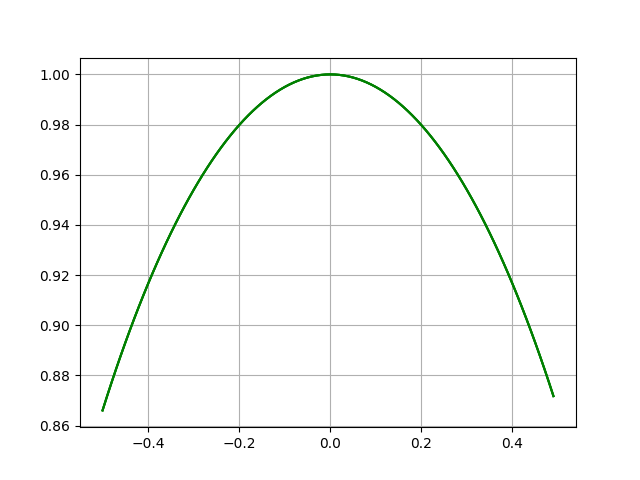
\includegraphics[scale=0.5]{Courbef.png}
\end{center}

Nous avons commencé par définir la fonction $f(x)$ à l'aide de la fonction \texttt{sqrt()} du module \texttt{math}. 
Après avoir représenté graphiquement la fonction sur l'intervalle $[-0.5, 0.5]$ nous avons calculé l'integrale suivante à la main : $$I=\int_{-0.5}^{0.5} \sqrt{1-x^2} \, \mathrm{d}x $$ (voir annexe papier)


\section{EXERCICE :  méthode du point milieu}

Calcul approché de $I$ au moyen de la {\bf méthode du point milieu}. Pour mieux se repérer, nous avons représenter graphiquement f sur papier. (voir annexe)

Ensuite, on va en premier temps définir une subdivision régulière $x0,x1,...,x4$ de l'intervalle d'intégration $[0,1]$ en n= 4 parts égales. 

En deuxième temps on définit les milieux de ces sous-intervalles. Avec ces données on calcule la surface $s{k}$ du rectanggle de base $[x{k-1},x{k}]$ et de hauteur $f(c{k})$. On sait que la surface d'un rectangle est $S= b*h$ avec b la base et h la hauteur du rectangle.

La {\it méthode du point milieu} consiste à prendre la somme $S{4}=\sum_{i=1}^{4} (s_{k})$ comme approximation de $I$.
\\

Par la suite, il a fallut calculer l'erreur entre l'intégrale et l'approximation qu'on en a faite. Pour cela, on a calculer la valeur absolue de $S{4}$ soutrait à l'intégrale $I$.
\\

Nous avons également utiliser la fonction \texttt{clock()} du module \texttt{time} pour mesurer le temps de calcul de notre intégrale. 
\\

Puis nous avons eu à écrire la fonction {\it point milieu} qui utilise la {\it méthode du point milieu}. Pour pouvoir la tester par la suite avec $f(x) = \sqrt{1 - x^2}$, \texttt{a = -0.5}, \texttt{b = 0.5}, et \texttt{n} qui va de \texttt{10} à \texttt{1 000 000}. Et avoir la tableau suivant :
\\

\begin{center}
\begin{tabular}{r | c | c}
{n} & erreur & temps (sec.)\\
\hline
$10$ & {0.000480384} & {3.6e-05}\\
$100$ & {4.811178e-06} & {0.000184}\\
$1000$ & {4.81125e-08} & {0.001663}\\
$10000$ & {4.8113e-10} & {0.01584}\\
$100000$ & {4.81315e-12} & {0.161942}\\
$1000000$ & {5.06262e-14} & {1.57448}
\end{tabular}
\end{center}

\section{EXERCICE : méthode du trapèze}

	Pour la\textit{ méthode du trapèze}, on approxime \texttt{f} sur l'intervalle $[x{k-1},x{k}]$ par la fonction affine qui prend les mêmes valeurs que \texttt{f} en $x_{k-1}$ et $x_k$.\\

	On a essayé de calculer l'intégrale par la \textit{méthode du trapèze}. Pour cela, on définit la fonction \textit{trapeze} qui prend en arguments une fonction \texttt{f}, des bornes \texttt{a} et \texttt{b} et un entier \texttt{n} et qui renvoie l'intégrale approchée de \texttt{f} sur $[a,b]$ au moyen de la \textit{méthode du trapèze}.\\

	Puis on a testé la méthode de la même manière qu'avec la méthode du point milieu. \\ 

Avec les données acquises nous avons rempli le tableau ci-dessous:
\\

\begin{center}
\begin{tabular}{r | c | c}
{n} & erreur & temps (sec.)\\
\hline
$10$ & {0.000961402} & {2.1e-05}\\
$100$ & {9062242e-06} & {7.8e-05}\\
$1000$ & {9.6225e-08} & {0.00077}\\
$10000$ & {9.6225e-10} & {0.007611}\\
$100000$ & {9.63307e-12} & {0.076049}\\
$1000000$ & {1.11022e-13} & {0.744644}
\end{tabular}
\end{center}

\section{EXERCICE : Méthode de Simpson}

Pour la \textit{méthode de Simpson}, on approxime \texttt{f} sur l'intervalle $[x_{k-1}, x_k]$ par le polynôme de degré 2 qui prend les mêmes valeurs que \texttt{f} en $x_{k-1}$, $c_k$ et $x_k$.\\
Nous avons définit la \textit{fonction Simpson} à l'aide de nos camarades.\\ 

	Puis nous avons testé notre programmme également de la même manière que les méthodes précédentes.\\ 
	Avec ces données, nous avons rempli le tableau ci-dessous: \\

\begin{center}
\begin{tabular}{r | c | c}
{n} & erreur & temps (sec.)\\
\hline
$10$ & {2.11626e-07} & {2.8e-05}\\
$100$ & {2.13807e-11 } & {0.000185}\\
$1000$ & {1.33227e-15} & {0.002373}\\
$10000$ & {6.76126e-14} & {0.02393}\\
$100000$ & {6.27609e-13} & {0.239471}\\
$1000000$ & {1.12086e-11} & {2.40692}
\end{tabular}
\end{center}

\section{EXERCICE : comparaison des trois méthodes précédentes}

Les trois méthodes \textbf{point milieu, trapèze} et \textbf{simpson} nous permettent de calculer une approximation d'intégrale d'une fonction sur un intervalle. 
\\

	
	Il y a en revanche quelques différences entre ces méthodes. Dans la \textit{méthode du point milieu} on approxime \texttt{f} par la fonction constante , dans la \textit{méthode du Trapèze} on approxime par la fonction affine et dans la \textit{méthode de Simpson} on approxime par la fonction du polynôme de degré 2. 
\\

	On remarque que l'erreur commise est différente pour chaque méthode. On voit que la \textit{méthode de Simpson} est plus efficace que les deux autres méthodes. En effet les erreurs commises par la \textit{méthode de Simpson} sont très inférieures à celles des deux autres méthodes.

\section{EXERCICE : méthode de Monte-Carlo}

Nous avons eu du mal à dessiner le cercle unité ne sachant pas la fonction à utiliser sur Python, nous avons fait quelques recherches sur Internet puis la solution du problème a été trouvée. Le cercle tracé :

\begin{center}
    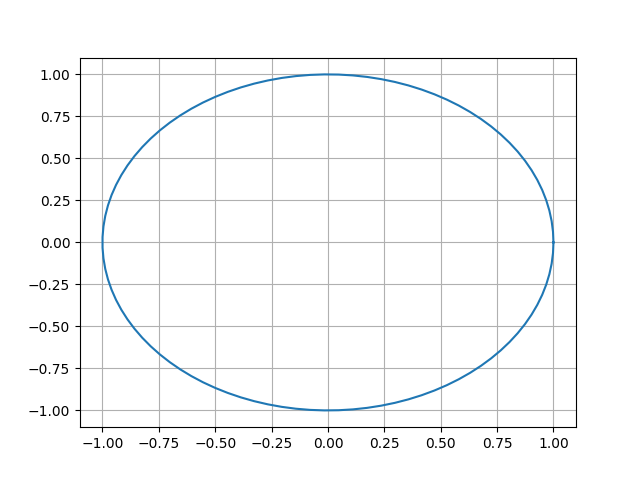
\includegraphics[width=0.65\textwidth]{CercleExo6(0).png}
\end{center}

Grâce à la fonction \textit{numpy.random.rand()}, nous avons généré quelques valeurs aléatoires représentées en \texttt{bleu} pour celles inférieures au disque unité et en \texttt{jaune} pour celles qui lui sont supérieures. Ces valeurs sont d'abord générées suivant la distribution de la loi uniforme sur $[0,1]$.  Ce qui nous donne le cercle suivant :

\begin{center}
    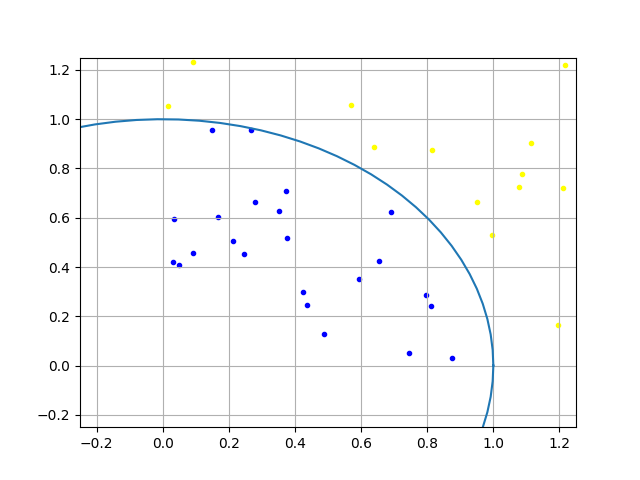
\includegraphics[width=0.65\textwidth]{CercleExo6(1).png}
\end{center}

 Puis suivant la distribution de la loi uniforme sur $[-1,1]$ : 

\begin{center}
    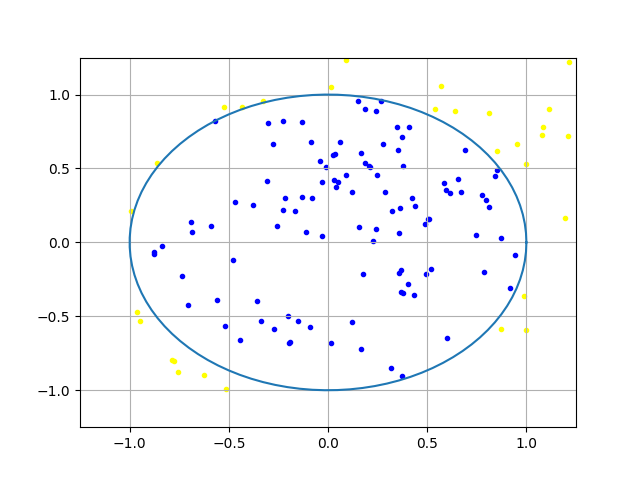
\includegraphics[width=0.65\textwidth]{CercleExo6(2).png}
\end{center}

\\
Puis nous avons généré \texttt{1000} points qui suivent la distribution uniforme sur le carré $[-1,1]^2$ et nous avons fait apparaître les points inférieurs au disque unité en rouge et les points extérieurs au disque en vert :

\begin{center}
    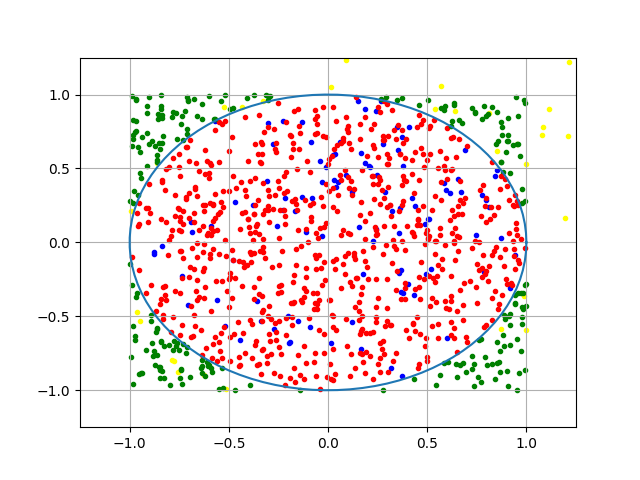
\includegraphics[width=0.65\textwidth]{CercleExo6(3).png}
\end{center}

Ensuite on a compté le nombre \texttt{I} de points intérieurs et le nombre \texttt{E} de points extérieurs. \\ 

	On sait que la \textit{méthode de Monte Carlo} consiste à prendre le rapport $\frac{I}{N}$ comme approximation de la surface \texttt{S} du disque. Ainsi nous avons calculé la valeur absolue du rapport $\frac{I}{N}$ soustrait à S pour savoir l'erreur commise par la fonction \textit{Monte Carlo}. On a utilisé \texttt{clock()} pour mesurer le temps de calcul.
\\

	On a testé la fonction \textit{Monte Carlo} avec $N=10^k$, k variant de 1 à 6.\\

	Monte Carlo est une fonction avec des valeurs aléatoire donc le tableau suivant change à chaque fois que le programme sera exécuté.\\

\begin{center}
\begin{tabular}{r | c | c}
{n} & erreur & temps (sec.)\\
\hline
$10$ & {0.0975927} & {7.8e-05}\\
$100$ & {0.0975927 } & {0.000256}\\
$1000$ & {0.0975927} & {0.002503}\\
$10000$ & {0.0975927} & {0.02528}\\
$100000$ & {0.0975927} & {0.246219}\\
$1000000$ & {0.0975927} & {2.47361}
\end{tabular}
\end{center}

Et enfin, nous avons défini une fonction \textit{monte\_carlo\_2} pour le calcul du volume de la boule unité.  




\end{document}



